\documentclass[../../main.tex]{subfiles}
\begin{document}

\subsection*{8.1}
Una bobina rigida quadrata di lato a = 2cm, formata da N = 20 spire compatte, e percorsa da una corrente $i_b = 2A$ ed è posta a distanza y da un filo indefinito percorso da una corrente i = 50A.
\\Calcolare la forza magnetica $\vec{F}(y) $ che agisce sulla bobina dimostrando che per $y \gg a$, $F=\frac{mdB}{dy}$, se m è il momento magnetico della bobina e B il campo del filo.
\\Calcolare inoltre il lavoro $W_1$ compiuto dalla forza magnetica per spostare la bobina da $y_1=1cm$ e $y_2 = 2cm$ e il lavoro $W_2$ compiuto dalla forza magnetica per ruotare di 180° la bobina, quando $y=y_4=20cm$.
\\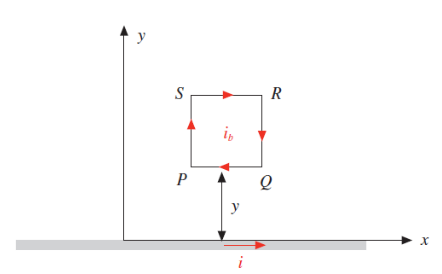
\includegraphics[scale=0.3]{e_8_1.png}
\subsubsection*{Formule utilizzate}
$\vec{F} = i\int_A^Bd\vec{j}\wedge\vec{B}$
\subsubsection*{Soluzione punto a}
il filo percorso da corrente i produce un campo $B = \frac{\mu_0\ i}{2\pi\ r}$ con direzione che sarà uscente al di sopra e entrante al di sotto dell'asse x.
\\in $\vec{PQ}$ il campo magnetico è pari a $B = \frac{\mu\ i}{2\pi y}$
\\in $\vec{SR}$ il campo magnetico è pari a $B = \frac{\mu\ i}{2\pi (y+a)}$
\\in $\vec{PS}$ la forza è opposta a quella di $\vec{RQ}$ quindi la forza risultante è nulla, poichè:
\\$\vec{F_{PS}} = \frac{i^2\mu_0}{2\pi}\int_P^S\frac{1}{y}dy$
\\$\vec{F_{RQ}} = \frac{i^2\mu_0}{2\pi}\int_R^Q\frac{1}{y}dy$
\\$\vec{F}(y) = \vec{F_{PQ}} + \vec{F_{RS}} = \frac{\mu_0\ N\ i\ i_b\ a}{2\ \pi}\left(\frac{1}{y}-\frac{1}{y+a}\right)\vec{u_y} = \frac{\mu_0\ N\ i\ i_b\ a^2}{2\ \pi\ y\ (y+a)}\vec{u_y}$
\\La forza ottenuta è repulsiva e questo è corente con $\vec{F} = N i_b \bigtriangleup\phi(\vec{B})$ dove $\phi(\vec{B})$ è il flusso del campo magnetico generato attraverso la bobina.
\\Se la spira si allontana il glusso di B diventa meno negativo, cioè aumenta.
\\Dato che la bobina percorsa da corrente $i_b$ ha area $Na^2$ il suo momento magnetico vale:
\\$vec{m} = -N\ i_b\ a^2\ \vec{u_z}$
\\mentre il filo percorso da una corrente i ad una distanza y produce un campo magnetico B che vale:
\\$\vec{B} = \frac{\mu_0\ i}{2\pi y}\vec{u_z}$
\\Si nota che: $\vec{F} = \bigtriangledown(\vec{m} * \vec{B}) = \bigtriangledown(mB_z) = m\frac{dB_z}{dy}\vec{u_y}$
\\$F(y) = m\frac{dB}{dy} = -Ni_ba^2\frac{d}{dy}\left[\frac{\mu_0\ i}{2\pi y}\right] = \frac{\mu_0\ N\ i\ i_b\ a^2}{2\pi y^2}$
\\$W_1 = \int_{y_1}^{y_2}Fdy = \frac{\mu_0Nii_ba}{2\pi}\int_{y_1}^{y_2}\left(\frac{1}{y}-\frac{1}{y+a}\right)dy = \frac{\mu_0Nii_ba}{2\pi}ln\left(\frac{y_2(y_1+a)}{y_1(y_2+a)}\right)$
\subsubsection*{Soluzione punto b}
$W_2 = \Delta U_p = U_p(f) - U_p(i) = -m\vec{i}*\vec{B}+\vec{mf}*\vec{B}$
\\$m =iS = ia^2 =mi=mf$
\newpage

\end{document}